\documentclass[11pt]{article}
\usepackage[utf8]{inputenc} 
\usepackage[T1]{fontenc}    
\usepackage{url}            
\usepackage{booktabs}       
\usepackage{amsfonts}       
\usepackage{nicefrac}       
\usepackage{microtype}      
\usepackage{fullpage}


\usepackage[numbers]{natbib}
%\usepackage[textsize=tiny]{todonotes}
\setlength{\marginparwidth}{11ex}

\newcommand{\E}{\mathbb E}
\usepackage{wrapfig}
\usepackage{caption}

\newcommand{\theHalgorithm}{\arabic{algorithm}}

\usepackage{url}

\usepackage[utf8]{inputenc}
\usepackage{amsmath}
\usepackage{graphicx}
\usepackage{upgreek}
\usepackage{amsfonts}
\usepackage{amssymb}
\usepackage{amsthm}
\usepackage[mathscr]{euscript}
\usepackage{mathtools}
\newtheorem{thm}{Theorem}
\newtheorem{defn}{Definition}
\newtheorem{cor}{Corollary}
\newtheorem{assumption}{Assumption}
\newtheorem{lem}{Lemma}
\usepackage{xcolor}
\usepackage{nicefrac}
\usepackage{xr}
%\usepackage{chngcntr}
\usepackage{apptools}
\usepackage[page, header]{appendix}
\AtAppendix{\counterwithin{lem}{section}}
\usepackage{titletoc}
\usepackage{enumitem}
\setlist[itemize]{leftmargin=1cm}
\setlist[enumerate]{leftmargin=1cm}




\definecolor{DarkRed}{rgb}{0.75,0,0}
\definecolor{DarkGreen}{rgb}{0,0.5,0}
\definecolor{DarkPurple}{rgb}{0.5,0,0.5}
\definecolor{Dark}{rgb}{0.5,0.5,0}
\definecolor{DarkBlue}{rgb}{0,0,0.7}
\usepackage[bookmarks, colorlinks=true, plainpages = false, citecolor = DarkBlue, urlcolor = blue, filecolor = black, linkcolor =DarkGreen]{hyperref}
\usepackage{breakurl}
\usepackage[ruled, vlined, linesnumbered]{algorithm2e}
\newcommand\mycommfont[1]{\footnotesize\ttfamily\textcolor{blue}{#1}}
\SetCommentSty{mycommfont}

\DeclareMathOperator*{\argmin}{arg\,min}
\DeclareMathOperator*{\argmax}{arg\,max}

\allowdisplaybreaks[2]
\newcommand{\prob}{\mathbb P}
\newcommand{\Var}{\mathbb V}
\newcommand{\Ex}{\mathbb E}
\newcommand{\varV}{\mathscr V}
\newcommand{\indicator}[1]{\mathbb I\{ #1 \} }
\newcommand{\statespace}{\mathcal S}
\newcommand{\actionspace}{\mathcal A}
\newcommand{\saspace}{\statespace \times \actionspace}
\newcommand{\satspace}{\mathcal Z}
\newcommand{\numsa}{\left|\saspace\right|}
\newcommand{\numsat}{\left|\satspace\right|}
\newcommand{\numS}{S}
\newcommand{\numA}{A}
\newcommand{\wmin}{w_{\min}}
\newcommand{\wminc}{w'_{\min}}
\newcommand{\range}{\operatorname{rng}}
\newcommand{\polylog}{\operatorname{polylog}}
\newcommand{\dspace}{\mathcal D}
\newcommand{\numD}{|\dspace|}
\newcommand{\numSucc}[1]{|\statespace(#1)|}
\newcommand{\succS}[1]{\statespace(#1)}

\newcommand{\reals}{\mathbb R}
\newcommand{\const}{\textrm{const.}}
\newcommand{\set}[1]{\left\{#1\right\}}
\newcommand{\llnp}{\operatorname{llnp}}
\newcommand{\defeq}{:=}
\usepackage{xspace}
\newcommand{\algname}{UBEV\xspace}

\mathtoolsset{showonlyrefs=true}

\let\temp\epsilon
\let\epsilon\varepsilon
\newcommand{\cK}{\mathcal K}
\newcommand{\cI}{\mathcal I}
\newcommand{\Pro}{\mathbb P}

\title{CS 234 Winter 2018 \\ Assignment 1 \\ Due: January 23 at 11:59 pm}
\date{}

\begin{document}
	\maketitle
\noindent For submission instructions please refer to \href{http://web.stanford.edu/class/cs234/assignments.html}{website}

\section{Optimal Policy for Simple MDP [20 pts]}

Consider the simple $n$-state MDP shown in Figure \ref{fig:Q1}. Starting from state $s_1$, the agent can move to the right ($a_0$) or left ($a_1$) from any state $s_i$. Actions are deterministic and always succeed (e.g. going left from
state $s_2$ goes to state $s_1$, and going left from state $s_1$ transitions to itself). Rewards are given upon taking an action from the state. Taking any action from the goal state $G$ earns a reward of $r=+1$
and the agent stays in state $G$. Otherwise, each move has zero reward ($r=0$). Assume a discount factor $\gamma < 1$.

\begin{figure}[h]
  \centering
    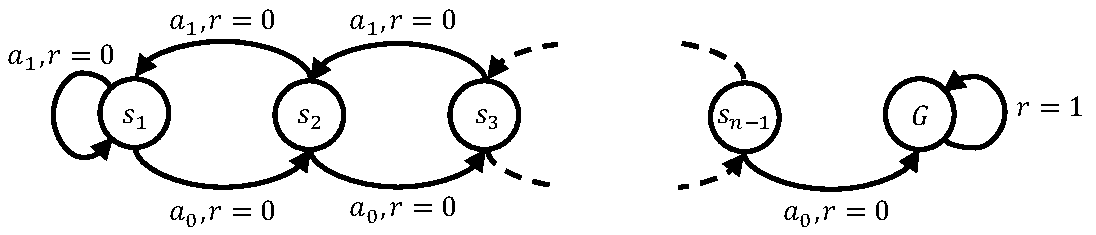
\includegraphics[width=0.5\textwidth]{Q1.pdf}
    \caption{$n$-state MDP}
  	\label{fig:Q1}
\end{figure}

\begin{enumerate}[label=(\alph*)]
\item The optimal action from any state $s_i$ is taking $a_0$ (right) until the agent reaches the goal state $G$. Find the optimal value function for all states $s_i$ and the goal state $G$. [5 pts]


\item Does the optimal policy depend on the value of the discount factor $\gamma$? Explain your answer. [5 pts]

\item Consider adding a constant $c$ to all rewards (i.e. taking any action from states $s_i$ has reward $c$ and any action from the goal state $G$ has reward $1+c$). Find the new optimal value function for all states $s_i$ and the goal state $G$. Does adding a constant reward $c$ change the optimal policy? Explain your answer. [5 pts]

\item After adding a constant $c$ to all rewards now consider scaling all the rewards by a constant $a$ (i.e. $r_{new} = a(c+ r_{old})$). Find the new optimal value function for all states $s_i$ and the goal state $G$. Does that change the optimal policy? Explain your answer, If yes, give an example of $a$ and $c$ that changes the optimal policy. [5 pts]

\end{enumerate}



\section{Running Time of Value Iteration [20 pts]}
In this problem we construct an example to bound the number of steps it will take to find the optimal policy using value iteration. Consider the infinite MDP with discount factor $\gamma < 1$ illustrated in Figure \ref{fig:Q2}. It consists of 3 states, and rewards are given upon taking an action from the state. From state $s_0$, action $a_1$ has zero immediate reward and causes a deterministic transition to state $s_1$ where there is reward $+1$ for every time step afterwards (regardless of action). From state $s_0$, action $a_2$ causes a deterministic transition to state $s_2$ with immediate reward of $\gamma^2/(1-\gamma)$ but state $s_2$ has zero reward for every time step afterwards (regardless of action).

\begin{figure}[h]
  \centering
    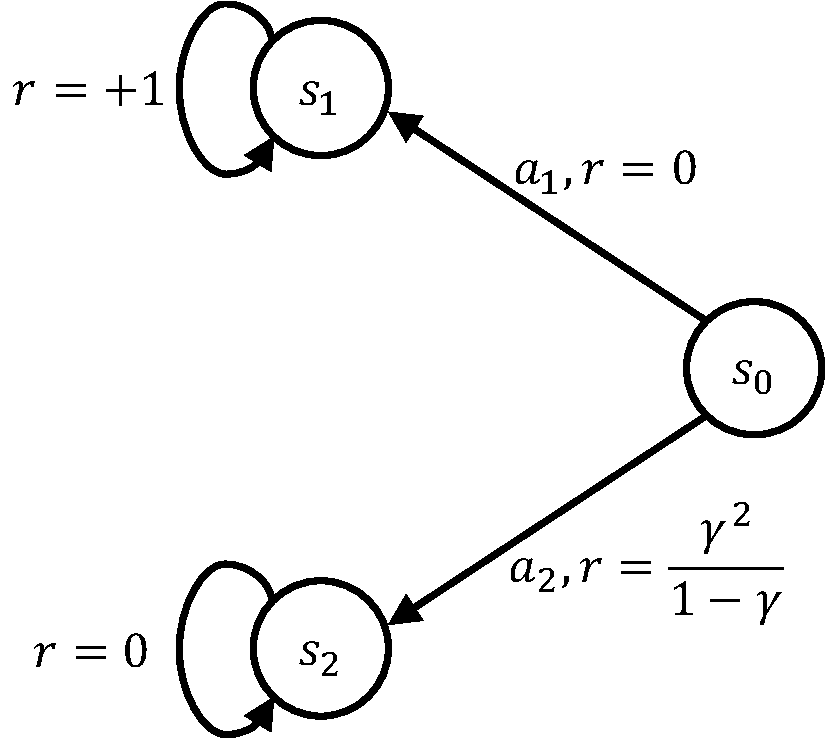
\includegraphics[width=0.3\textwidth]{Q2.pdf}
    \caption{infinite 3-state MDP}
  	\label{fig:Q2}
\end{figure}

\begin{enumerate}[label=(\alph*)]
\item What is the total discounted return ($\sum_{t=0}^{\infty}\gamma^t r_t$) of taking action $a_1$ from state $s_0$ at time step $t=0$? [5 pts]


\item What is the total discounted return ($\sum_{t=0}^{\infty}\gamma^t r_t$) of taking action $a_2$ from state $s_0$ at time step $t=0$? What is the optimal action? [5 pts]


\item Assume we initialize value of each state to zero, (i.e. at iteration $n=0$, $\forall s: V_{n=0}(s) = 0$). Show that value iteration continues to choose the sub-optimal action until iteration $n^*$ where, 
$$n^* \geq \frac{\log(1-\gamma)}{\log\gamma} \geq \frac{1}{2} \log (\frac{1}{1-\gamma})\frac{1}{1-\gamma}$$
Thus, value iteration has a running time that grows faster than $1/(1-\gamma)$. (You just need to show the first inequality) [10 pts]


\end{enumerate}

\section{Approximating the Optimal Value Function [35 pts]}
Consider a finite MDP $M=\langle S, A, T, R, \gamma \rangle$, where $S$ is the state space, $A$ action space, $T$ transition probabilities, $R$ reward function and $\gamma$ the discount factor. Define $Q^*$ to be the optimal state-action value $Q^*(s,a) = Q_{\pi^*}(s,a)$ where $\pi^*$ is the optimal policy. Assume we have an estimate $\tilde{Q}$ of $Q^*$, and $\tilde{Q}$ is bounded by $l_{\infty}$ norm as follows:

\begin{equation}
||\tilde{Q} - Q^*||_{\infty} \leq \epsilon
\end{equation}

\noindent Where $||x||_{\infty} = max_{s,a} |x(s,a)|$.\\

\noindent Assume that we are following the greedy policy with respect to $\tilde{Q}$, $\pi(s) = argmax_{a\in \mathcal{A}} \tilde{Q}(s,a)$. We want to show that the following holds:

\begin{equation}\label{eq:Q3} 
V_{\pi}(s) \geq V^*(s) - \frac{2\epsilon}{1-\gamma}
\end{equation}
\noindent Where $V_{\pi}(s)$ is the value function of the greedy policy $\pi$ and $V^*(s)=max_{a \in A} Q^*(s,a)$ is the optimal value function. This shows that if we compute an approximately optimal state-action value
function and then extract the greedy policy for that approximate state-action value
function, the resulting policy still does well in the real MDP.

\begin{enumerate}[label=(\alph*)]
\item Let $\pi^*$ be the optimal policy, $V^*$ the optimal value function and as defined above $\pi(s) = argmax_{a\in A} \tilde{Q}(s,a)$. Show the following bound holds for all states $s \in S$. [10 pts]

$$V^*(s) - Q^*(s, \pi(s)) \leq 2 \epsilon$$


\item Using the results of part 1, prove that $V_{\pi}(s) \geq V^*(s) - \frac{2\epsilon}{1-\gamma}$. [10 pts]


\end{enumerate}

\noindent Now we show that this bound is tight. Consider the 2-state MDP illustrated in figure \ref{fig:Q3}. State $s_1$ has two actions, "$stay$" self transition with reward 0 and "$go$" that goes to state $s_2$ with reward $2\epsilon$. State $s_2$ transitions to itself with reward $2\epsilon$ for every time step afterwards.

\begin{figure}[h]
  \centering
    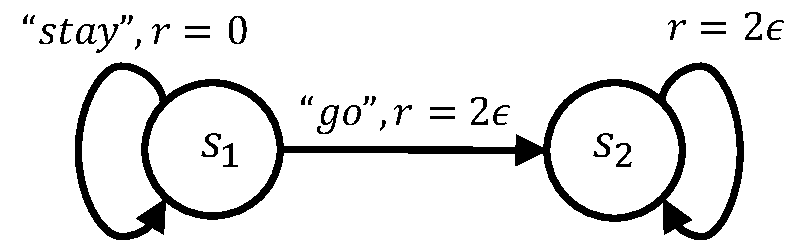
\includegraphics[width=0.3\textwidth]{Q3.pdf}
    \caption{2-state MDP}
  	\label{fig:Q3}
\end{figure}
\begin{enumerate}

\item[(c)] Compute the optimal value fucntion $V^*(s)$ for each state and the optimal state-action value function $Q^*(s,a)$ for state $s_1$ and each action. [5 pts]



\item[(d)] Show that there exists an approximate state-action value function $\tilde{Q}$ with $\epsilon$ error (measured with $l_{\infty}$ norm), such that $V_{\pi}(s_1) - V^*(s_1) = - \frac{2\epsilon}{1-\gamma}$, where $\pi(s) = argmax_{a \in A} \tilde{Q}(s,a)$. (You may need to define a consistent tie break rule) [10 pts]


\end{enumerate}

\begin{section}{Frozen Lake MDP [25 pts]}
Now you will implement value iteration and policy iteration for the Frozen Lake environment
from \href{"https://gym.openai.com/envs/FrozenLake-v0"}{OpenAI Gym}. We have provided
custom versions of this environment in the starter code.
\begin{enumerate}[label=(\alph*)]
\item \textbf{(coding)} Read through \texttt{vi\_and\_pi.py} and implement \texttt{policy\_evaluation}, \texttt{policy\_improvement} and \texttt{policy\_iteration}. The stopping tolerance (defined as $\max_s |V_{old}(s) - V_{new}(s)|$) is tol = $10^{-3}$
. Use $\gamma = 0.9$. Return the optimal value function and the optimal policy. [10pts]
\item \textbf{(coding)} Implement \texttt{value\_iteration} in \texttt{vi\_and\_pi.py}. The stopping tolerance is tol =
$10^{-3}$
. Use $\gamma = 0.9$. Return the optimal value function and the optimal policy. [10 pts]
\item \textbf{(written)} Run both methods on the Deterministic-4x4-FrozenLake-v0 and

Stochastic-4x4-FrozenLake-v0 environments. In the second environment, the dynamics of the world are stochastic. How does stochasticity affect the number of iterations required, and the resulting policy? [5 pts]

\end{enumerate}
\end{section}

\end{document} 
